\documentclass[12pt]{article}
\usepackage{latexsym}
\usepackage{epsfig}
\usepackage{amsmath}
\usepackage{amssymb}


\setlength{\topmargin}{0in}
\setlength{\leftmargin}{0in}
\setlength{\textwidth}{6in}
\setlength{\textheight}{9.5in}
\setlength{\parindent}{0.2in}
\setlength{\parskip}{.08in}
\voffset = -.45in
\hoffset = -.5in
\def\filledbox{\vrule height 1.8ex width .8ex depth -.1ex } % square bullet
\newcommand{\qed}{\large ~$\Box$ \normalsize}
%
%\newtheorem{thm}{Theorem}
%\newenvironment{theorem}{\begin{thm}\ \rm}{\end{thm}}
%
%\newtheorem{lem}{Lemma}
%\newenvironment{lemma}{\begin{lem}\ \rm}{\end{lem}}
%
\newtheorem{theorem}{Theorem}
\newtheorem{lemma}{Lemma}
\newtheorem{corollary}{Corollary}
\newenvironment{proof}{{\noindent \bf Proof\ \ }}{\qed}
\newenvironment{proofsketch}{{\noindent {\bf Proof}\ (sketch)\ \ }}{\qed}
%
\def\shh{\skew3\hat{\hat s}}
\def\dhh{\skew6\hat{\hat d}}
\begin{document}
\newcommand{\I}{\mbox{{\em Int}}}
\newcommand{\lt}{\mbox{{\em left}}}
\newcommand{\rt}{\mbox{{\em right}}}
\newcommand{\ld}{\Delta^l}
\newcommand{\rd}{\Delta^r}
\newcommand{\lsp}[1]{\large\renewcommand{\baselinestretch}{#1}\normalsize}
\newcommand{\hsp}{\hspace{.2in}}

\def\Endwhile{\mbox{\bf endwhile\ }}
\def\Or{\mbox{\bf or\ }}
\def\Do{\mbox{\bf do\ }}
\def\Downto{\mbox{\bf downto\ }}
\def\Int{\mbox{\bf int\ }}
\def\To{\mbox{\bf to\ }}
\def\Repeat{\mbox{\bf repeat\ }}
\def\Until{\mbox{\bf until\ }}
\def\Return{\mbox{\bf return\ }}
\def\Not{\mbox{\bf not\ }}
\def\And{\mbox{\bf and\ }}
\def\For{\mbox{\bf for\ }}
\def\Foreach{\mbox{\bf foreach\ }}
\def\Else{\mbox{\bf else\ }}
\def\Elseif{\mbox{\bf elseif\ }}
\def\End{\mbox{\bf end\ }}
\def\If{\mbox{\bf if\ }}
\def\Mod{\mbox{\bf \ mod\ }}
\def\Then{\mbox{\bf then\ }}
\def\While{\mbox{\bf while\ }}
\def\Output{\mbox{\bf output\ }}


\lsp{1}
\pagestyle{plain}
\begin{center}
{\bf
Dijkstra Worksheet
}
\end{center}

\begin{figure}[h]
\center
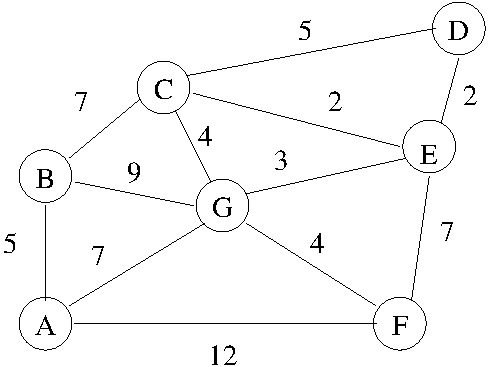
\includegraphics[width = 3in]{spanning.pdf}
\end{figure}

Execute Dijkstra's algorithm on the provided graph starting
at vertex $A$. Indicate which vertex was selected at each 
iteration of the {\bf while} loop and show the contents of
the priority queue.

\begin{description}
\item [Final Distances]\ 

\begin{tabular}{|c|c|}\hline
A:0 & E:10\\\hline
B:5 & F:11\\\hline
C:11  & G:7\\\hline
D:12  & \\\hline
\end{tabular}
\item [Iteration 1]\ 

$u =$\ A

$S = \{$A\}

Queue:\\
\begin{tabular}{|c|c|}\hline
                & E:$\infty$\\\hline
    B:5         & F:12\\\hline
    C:$\infty$  & G:7\\\hline
    D:$\infty$  & \\\hline
\end{tabular}
\item [Iteration 2]\ 

$u =$\ B

$S = \{$A, B\}

Queue:\\
\begin{tabular}{|c|c|}\hline
                & E:$\infty$\\\hline
                & F:12\\\hline
    C:12        & G:7\\\hline
    D:$\infty$  & \\\hline
\end{tabular}

\item [Iteration 3]\ 

$u =$\ G

$S = \{$A, B, G\}

Queue:\\
\begin{tabular}{|c|c|}\hline
                & E:10\\\hline
                & F:11\\\hline
    C:11        & \\\hline
    D:$\infty$  & \\\hline
\end{tabular}
\item [Iteration 4]\ 

$u =$\ E

$S = \{$A, B, G, E\}

Queue:\\
\begin{tabular}{|c|c|}\hline
                & \\\hline
                & F:11\\\hline
    C:11        & \\\hline
    D:12        & \\\hline
\end{tabular}
\item [Iteration 5]\ 

$u =$\ C

$S = \{$A, B, G, E, C\}

Queue:\\
\begin{tabular}{|c|c|}\hline
                & \\\hline
                & F:11\\\hline
                & \\\hline
    D:12        & \\\hline
\end{tabular}
\item [Iteration 6]\ 

$u =$\ F

$S = \{$A, B, G, E, C, F\}

Queue:\\
\begin{tabular}{|c|c|}\hline
                & \ \ \ \ \ \ \\\hline
                & \\\hline
                & \\\hline
    D:12        & \\\hline
\end{tabular}
\end{description} 



\end{document}
